% There should be a better way to program vector graphics in LaTeX

\begin{figure}
\centering

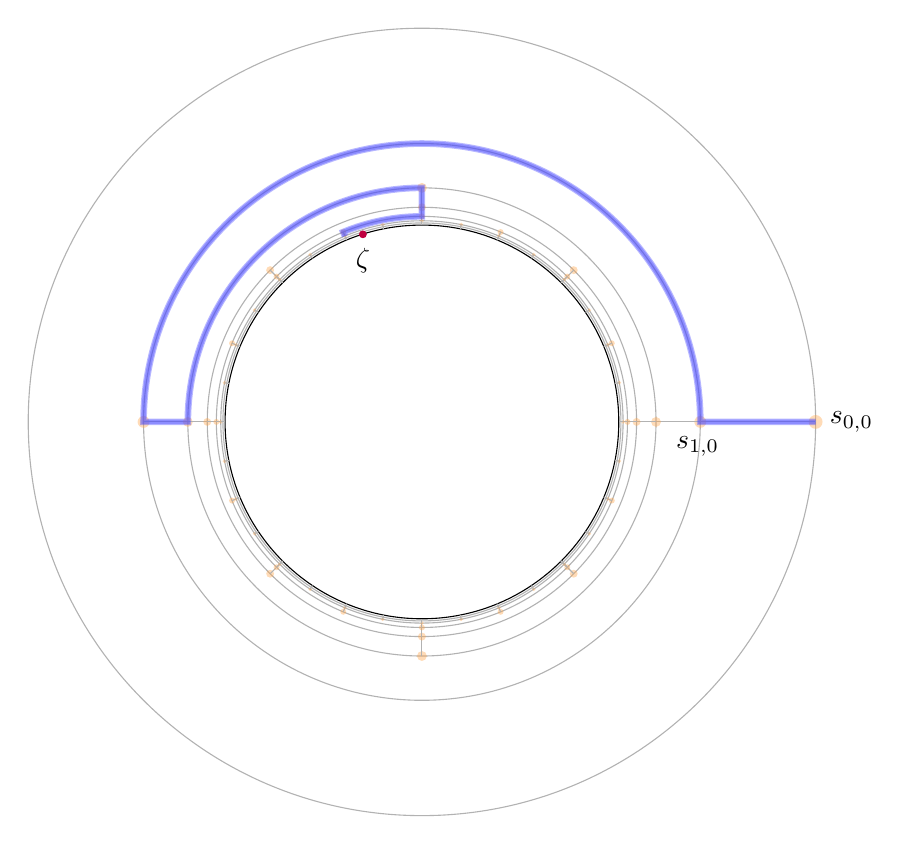
\begin{tikzpicture}[scale=2.5]
		
% The circles C_n
\draw (0,0) circle (1);
\foreach \i in {1,(1.0/2),(1.0/4),(1.0/8), (1.0/16), (1.0/32), (1.0/64)}{
\draw[black!30!white] (0,0) circle (2^\i);
}
   
\foreach \j in {0,1,2,3,4,5}{
    \pgfmathsetmacro{\jtwo}{2.0^\j}
    \pgfmathsetmacro{\jthree}{(1.0/\jtwo)}
    \pgfmathsetmacro{\twopower}{2^\jthree}
    \foreach \angleone in {1,...,\jtwo}{
    \pgfmathsetmacro{\anglez}{360*\angleone}
    \pgfmathsetmacro{\size}{1-\j/7.0}
    \fill[orange!70!white] (\anglez * \jthree: \twopower) circle (\size pt)[opacity=0.4];
    \draw[black!30!white] (\anglez * \jthree: \twopower) -- (\anglez * \jthree: 1);	
    }
}	


% The central itinerary
\draw [blue!70!white,-,
	double=blue!70!white,
	double distance=4\pgflinewidth, opacity=0.4,
	] 
    (2,0) 
 -- (2^0.5,0) 
 arc (0:180:2^0.5) 
 -- (-2^0.25,0) 
 arc (180:90:2^0.25)
 -- (0,2^0.0625)
 arc (90:112.5:2^0.0625)
 --(112.5:2^0.03125);


\node[circle,inner sep=1pt,fill=purple,label=below:{$\zeta$}] at (-0.3,0.953) {};

\node[circle,inner sep=1pt,label=right:{$s_{0,0}$}] at (2,0) {};

\node[circle,inner sep=1pt,label=below:{$s_{1,0}$}] at (1.4,0) {};

\end{tikzpicture}

\caption{The central itinerary to a point $\zeta$.} 
\label{fig:Carleson1}
\end{figure}
